% Matthias
\section{Spielideen}
Bei der Spielidee war es uns wichtig, auf der einen Seite einen interessanten
und wirtschaftlich herausfordernden Markt darzustellen und auf der anderen Seite
dem Spieler das Gef�hl zu geben, ein Spiel zu spielen.\\
W�hrend der erste Punkt eine gewisse Recherche m�glicher M�rkte beinhaltet, geht
es beim zweiten vielmehr darum, typische Mechaniken eines Spiels zu
implementieren.

Im Folgenden werden die beiden Punkte genauer untersucht:
\subsection{Der Markt des Spiels: Strommarkt}
Bei der Analyse unterschiedlicher M�rkte haben sich einige Eigenschaften
herausgestellt, die f�r die Realisierung eines m�glichen Spiels entscheidend
waren:

\begin{itemize}
  \item \textbf{Oligopol}: Da jeder Spieler die M�glichkeit haben soll,
  den Markt zu beeinflussen, sollte es kein Massenmarkt mit hunderten Anbietern
  sein. Tats�chlich ist es f�r einen Spieler ein weitaus intensiveres
  Spielerlebnis, wenn er sich selbst als relevanten --- wenn nicht sogar
  essentiellen --- Marktteilnehmer sieht.
  \item \textbf{Produktionssektor}: Auch wenn es gewiss einen gewissen Charme
  h�tte, ein Unternehmen des Dienstleistungssektors abzubilden, fiel bei diesem
  Spiel die Entscheidung, das Unternehmen im prim�ren Sektor anzusiedeln. Das
  hat den Vorteil, dass sich elementare marktbegrenzende Mechanismen wie
  Ressourcenknappheit oder begrenzte Nachfrage simulieren lassen.
  \item \textbf{Differenzierter Markt / differenzierte Produktion}: Ein weiterer
  Fokus lag darauf, dass dem Spieler Handlungsfreiheiten gegeben werden sollen,
  die nicht nur darin bestehen, die Kosten f�r einzelne Abteilungen und den
  Preis f�r das Endprodukt einzustellen, sondern ihm auch eine gewisse
  Diversifikation und damit die M�glichkeit einer Ausarbeitung von verschiedenen
  Strategien zur Hand zu geben. Dies lie�e sich einerseits durch einen Markt mit
  mehreren klar differenzierbaren Produkten (z.B. Smartphone und Tablet) als
  auch durch eine mehrstufige Produktionskette realisieren. (Mit der
  M�glichkeit, nur manche Abschnitte der Wertsch�pfungskette selbst abzubilden.)
\end{itemize}

Als interessantester und vielversprechendster Markt hat sich schlie�lich der
Energiemarkt --- in diesem Fall der Strommarkt --- herauskristallisiert. Das
Oligopol ist hier insofern gegeben, als dass die vier gr��ten Stromproduzenten
in Deutschland (E.ON, RWE, EnBW und Vattenfall) einen Marktanteil von 80\%
abdecken.

Um nun auch ein Mindestma� an Handlungsfreiheit zu gew�hrleisten, wurde beim
Spielkonzept nicht nur der Wertsch�pfungsaspekt der direkten Stromproduktion
durch Kraftwerke betrachtet, sondern auch die Gewinnung der daf�r erforderlichen
Ressourcen. Es liegt am Spieler, zu entscheiden, ob es am lukrativsten ist, die
erforderlichen Ressourcen in Minen abzubauen oder diese direkt am Markt zu
kaufen. Dar�ber hinaus stehen dem Spieler durch die Wahl zwischen diversen
fossilen Brennstoffen (Gas, Uran (Kernenergie), Kohle) und erneuerbaren Energien
(Wind, Wasser, Solar) einige Aspekte der unternehmerischen Entscheidungsfindung
zur Verf�gung.

\begin{figure}[H]
\centering
\centering
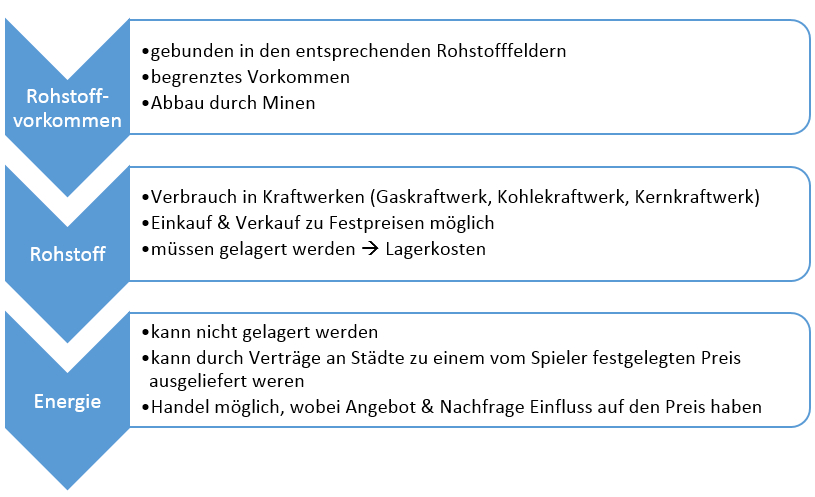
\includegraphics[width=0.8\textwidth]{se-wa-jpg/produktionskette}
\caption{Produktionskette}
\label{Produktionskette}
\end{figure}

Ein weiterer Aspekt ist, dass der Kauf von Kraftwerken immer eine hohe
Investition darstellt und damit eine hohe Tragweite hat, der Spieler also nicht
dazu gezwungen ist, jede Runde viele Investitionen zu t�tigen, um sein Kapital
sinnvoll binden zu k�nnen. Im Gegenteil: Der Spieler wird dazu forciert,
einige wenige (im Idealfall wohl �berlegte) Entscheidungen zu treffen, die entscheidend
f�r den weiteren Spielverlauf sein k�nnen.
\subsection{Das Spielprinzip}
Neben dem zu realisierenden Markt lag ein gro�er Fokus auf der Modellierung
dieses Marktes in einem geeigneten Modell, das auf der einen Seite sowohl den
Markt in seinen Grundz�gen abbildet, auf der anderen Seite aber auch einen hohen
Wert auf Spielspa� und Spielbarkeit legt.\\
Dazu sollte das Unternehmen vor allem nicht nur in Zahlen greifbar sein.
Investitionen (z.B. in ein neues Kraftwerk) sollen dem Spieler auch ein
Erfolgserlebnis bescheren, das ihm am besten auch visuell schmackhaft gemacht
wird.

F�r diese Ziele musste nun eine geeignete Abbildung in ein Spielkonzept gefunden
werden. Inspiriert vom Brettspielklassiker "`Die Siedler von Catan"' und
dem rundenbasierten Globalstrategiespiel "`Sid Meier's Civilization V"'
kam die Idee eines Sechseckrasters als "`Spielfeld"' auf. Dies
erm�glicht eine Visualisierung des Grundgeschehens und zus�tzliche
Handlungsfreiheiten, da der Spieler entscheiden kann, welches Feld er wo kauft.

Um die Spielmechaniken nicht noch weiter zu verkomplizieren und dem Spieler
einen gewissen �berblick zu lassen, wurde auf ein rundenbasiertes Spielmodell
gesetzt.

% Wordcount: 610